\documentclass{standalone}
\usepackage{tikz}
\usetikzlibrary{patterns, positioning}


\begin{document}
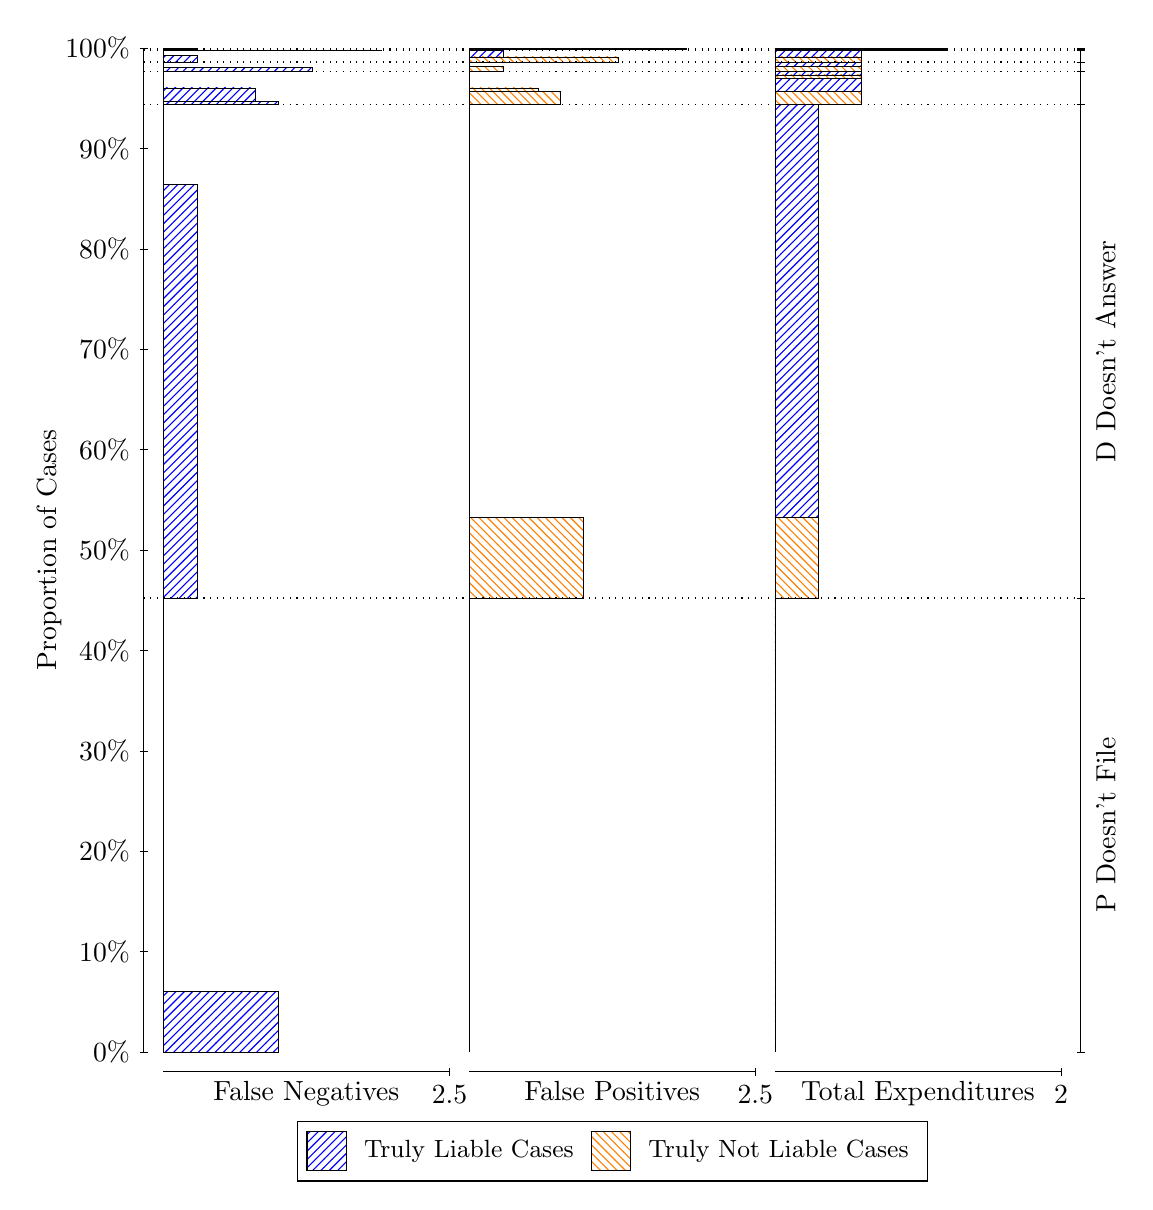
\begin{tikzpicture}
\draw[black, very thin] (1.5,1.75) -- (1.5,14.5);
\node[rotate=90, text=black, anchor=center] at (0.3, 8.125) {Proportion of Cases};
\draw[black, very thin] (1.45,1.75) -- (1.55,1.75);
\node[text=black, anchor=east] at (1.45, 1.75) {0\%};
\draw[black, very thin] (1.45,3.025) -- (1.55,3.025);
\node[text=black, anchor=east] at (1.45, 3.025) {10\%};
\draw[black, very thin] (1.45,4.3) -- (1.55,4.3);
\node[text=black, anchor=east] at (1.45, 4.3) {20\%};
\draw[black, very thin] (1.45,5.575) -- (1.55,5.575);
\node[text=black, anchor=east] at (1.45, 5.575) {30\%};
\draw[black, very thin] (1.45,6.85) -- (1.55,6.85);
\node[text=black, anchor=east] at (1.45, 6.85) {40\%};
\draw[black, very thin] (1.45,8.125) -- (1.55,8.125);
\node[text=black, anchor=east] at (1.45, 8.125) {50\%};
\draw[black, very thin] (1.45,9.4) -- (1.55,9.4);
\node[text=black, anchor=east] at (1.45, 9.4) {60\%};
\draw[black, very thin] (1.45,10.675) -- (1.55,10.675);
\node[text=black, anchor=east] at (1.45, 10.675) {70\%};
\draw[black, very thin] (1.45,11.95) -- (1.55,11.95);
\node[text=black, anchor=east] at (1.45, 11.95) {80\%};
\draw[black, very thin] (1.45,13.225) -- (1.55,13.225);
\node[text=black, anchor=east] at (1.45, 13.225) {90\%};
\draw[black, very thin] (1.45,14.5) -- (1.55,14.5);
\node[text=black, anchor=east] at (1.45, 14.5) {100\%};

\draw[black, very thin] (13.4,1.75) -- (13.4,14.5);
\draw[black, very thin] (13.35,1.75) -- (13.45,1.75);
\node[anchor=west] at (13.35, 1.75) {};
\draw[black, very thin] (13.35,7.5161) -- (13.45,7.5161);
\node[anchor=west] at (13.35, 7.5161) {};
\draw[black, very thin] (13.35,13.785) -- (13.45,13.785);
\node[anchor=west] at (13.35, 13.785) {};
\draw[black, very thin] (13.35,14.2) -- (13.45,14.2);
\node[anchor=west] at (13.35, 14.2) {};
\draw[black, very thin] (13.35,14.322) -- (13.45,14.322);
\node[anchor=west] at (13.35, 14.322) {};
\draw[black, very thin] (13.35,14.469) -- (13.45,14.469);
\node[anchor=west] at (13.35, 14.469) {};
\draw[black, very thin] (13.35,14.487) -- (13.45,14.487);
\node[anchor=west] at (13.35, 14.487) {};
\draw[black, very thin] (13.35,14.5) -- (13.45,14.5);
\node[anchor=west] at (13.35, 14.5) {};

\draw[black, very thin, pattern color=blue, pattern=north east lines] (1.75,1.75) rectangle (3.2033,2.5235);
\draw[black, very thin, pattern color=orange, pattern=north west lines] (1.75,2.5235) rectangle (1.75,7.5161);
\draw[black, very thin, pattern color=blue, pattern=north east lines] (1.75,7.5161) rectangle (2.186,12.765);
\draw[black, very thin, pattern color=orange, pattern=north west lines] (1.75,12.765) rectangle (1.75,13.785);
\draw[black, very thin, pattern color=blue, pattern=north east lines] (1.75,13.785) rectangle (3.2033,13.826);
\draw[black, very thin, pattern color=blue, pattern=north east lines] (1.75,13.826) rectangle (2.9127,13.993);
\draw[black, very thin, pattern color=orange, pattern=north west lines] (1.75,13.993) rectangle (1.75,14.2);
\draw[black, very thin, pattern color=blue, pattern=north east lines] (1.75,14.2) rectangle (3.6393,14.251);
\draw[black, very thin, pattern color=orange, pattern=north west lines] (1.75,14.251) rectangle (1.75,14.322);
\draw[black, very thin, pattern color=blue, pattern=north east lines] (1.75,14.322) rectangle (2.186,14.403);
\draw[black, very thin, pattern color=orange, pattern=north west lines] (1.75,14.403) rectangle (1.75,14.469);
\draw[black, very thin, pattern color=blue, pattern=north east lines] (1.75,14.469) rectangle (4.5113,14.474);
\draw[black, very thin, pattern color=orange, pattern=north west lines] (1.75,14.474) rectangle (1.75,14.487);
\draw[black, very thin, pattern color=blue, pattern=north east lines] (1.75,14.487) rectangle (2.186,14.495);
\draw[black, very thin, pattern color=orange, pattern=north west lines] (1.75,14.495) rectangle (1.75,14.5);
\draw[black, very thin, pattern color=orange, pattern=north west lines] (5.6333,1.75) rectangle (5.6333,6.7426);
\draw[black, very thin, pattern color=blue, pattern=north east lines] (5.6333,6.7426) rectangle (5.6333,7.5161);
\draw[black, very thin, pattern color=orange, pattern=north west lines] (5.6333,7.5161) rectangle (7.0867,8.5364);
\draw[black, very thin, pattern color=blue, pattern=north east lines] (5.6333,8.5364) rectangle (5.6333,13.785);
\draw[black, very thin, pattern color=orange, pattern=north west lines] (5.6333,13.785) rectangle (6.796,13.952);
\draw[black, very thin, pattern color=orange, pattern=north west lines] (5.6333,13.952) rectangle (6.5053,13.993);
\draw[black, very thin, pattern color=blue, pattern=north east lines] (5.6333,13.993) rectangle (5.6333,14.2);
\draw[black, very thin, pattern color=orange, pattern=north west lines] (5.6333,14.2) rectangle (6.0693,14.271);
\draw[black, very thin, pattern color=blue, pattern=north east lines] (5.6333,14.271) rectangle (5.6333,14.322);
\draw[black, very thin, pattern color=orange, pattern=north west lines] (5.6333,14.322) rectangle (7.5227,14.388);
\draw[black, very thin, pattern color=blue, pattern=north east lines] (5.6333,14.388) rectangle (6.0693,14.469);
\draw[black, very thin, pattern color=orange, pattern=north west lines] (5.6333,14.469) rectangle (6.0693,14.482);
\draw[black, very thin, pattern color=blue, pattern=north east lines] (5.6333,14.482) rectangle (5.6333,14.487);
\draw[black, very thin, pattern color=orange, pattern=north west lines] (5.6333,14.487) rectangle (8.3947,14.492);
\draw[black, very thin, pattern color=blue, pattern=north east lines] (5.6333,14.492) rectangle (6.9413,14.5);
\draw[black, very thin, pattern color=orange, pattern=north west lines] (9.5167,1.75) rectangle (9.5167,6.7426);
\draw[black, very thin, pattern color=blue, pattern=north east lines] (9.5167,6.7426) rectangle (9.5167,7.5161);
\draw[black, very thin, pattern color=orange, pattern=north west lines] (9.5167,7.5161) rectangle (10.062,8.5364);
\draw[black, very thin, pattern color=blue, pattern=north east lines] (9.5167,8.5364) rectangle (10.062,13.785);
\draw[black, very thin, pattern color=orange, pattern=north west lines] (9.5167,13.785) rectangle (10.607,13.952);
\draw[black, very thin, pattern color=blue, pattern=north east lines] (9.5167,13.952) rectangle (10.607,14.119);
\draw[black, very thin, pattern color=orange, pattern=north west lines] (9.5167,14.119) rectangle (10.607,14.16);
\draw[black, very thin, pattern color=blue, pattern=north east lines] (9.5167,14.16) rectangle (10.607,14.2);
\draw[black, very thin, pattern color=orange, pattern=north west lines] (9.5167,14.2) rectangle (10.607,14.271);
\draw[black, very thin, pattern color=blue, pattern=north east lines] (9.5167,14.271) rectangle (10.607,14.322);
\draw[black, very thin, pattern color=orange, pattern=north west lines] (9.5167,14.322) rectangle (10.607,14.388);
\draw[black, very thin, pattern color=blue, pattern=north east lines] (9.5167,14.388) rectangle (10.607,14.469);
\draw[black, very thin, pattern color=orange, pattern=north west lines] (9.5167,14.469) rectangle (11.697,14.482);
\draw[black, very thin, pattern color=blue, pattern=north east lines] (9.5167,14.482) rectangle (11.697,14.487);
\draw[black, very thin, pattern color=orange, pattern=north west lines] (9.5167,14.487) rectangle (11.697,14.492);
\draw[black, very thin, pattern color=blue, pattern=north east lines] (9.5167,14.492) rectangle (11.697,14.5);
\draw[black, dotted] (1.5,7.5161) -- (13.4,7.5161);
\draw[black, dotted] (1.5,13.785) -- (13.4,13.785);
\draw[black, dotted] (1.5,14.2) -- (13.4,14.2);
\draw[black, dotted] (1.5,14.322) -- (13.4,14.322);
\draw[black, dotted] (1.5,14.469) -- (13.4,14.469);
\draw[black, dotted] (1.5,14.487) -- (13.4,14.487);
\draw[black, very thin] (1.75,1.5) -- (5.3833,1.5);
\node[text=black, anchor=north] at (3.5667, 1.5) {False Negatives};
\draw[black, very thin] (5.3833,1.45) -- (5.3833,1.55);
\node[text=black, anchor=north] at (5.3833, 1.45) {2.5};

\draw[black, very thin] (5.6333,1.5) -- (9.2667,1.5);
\node[text=black, anchor=north] at (7.45, 1.5) {False Positives};
\draw[black, very thin] (9.2667,1.45) -- (9.2667,1.55);
\node[text=black, anchor=north] at (9.2667, 1.45) {2.5};

\draw[black, very thin] (9.5167,1.5) -- (13.15,1.5);
\node[text=black, anchor=north] at (11.333, 1.5) {Total Expenditures};
\draw[black, very thin] (13.15,1.45) -- (13.15,1.55);
\node[text=black, anchor=north] at (13.15, 1.45) {2};

\node[text=black, centered, rotate=90] at (13.72, 4.633) {P Doesn't File};
\node[text=black, centered, rotate=90] at (13.72, 10.651) {D Doesn't Answer};






\draw (7.449999999999999,1.5) node[draw=none] (baseCoordinate) {};
\begin{scope}[align=center]
        \matrix[scale=0.5, draw=black, below=0.5cm of baseCoordinate, nodes={draw}, column sep=0.1cm]{
            \node[rectangle, draw, minimum width=0.5cm, minimum height=0.5cm, pattern color=blue, pattern=north east lines] {}; &
            \node[draw=none, font=\small, text=black] (B) {Truly Liable Cases}; &
            \node[rectangle, draw, minimum width=0.5cm, minimum height=0.5cm, pattern color=orange, pattern=north west lines] {}; &
            \node[draw=none, font=\small, text=black] (B) {Truly Not Liable Cases}; \\
            };
\end{scope}

\end{tikzpicture}
\end{document}